\documentclass[12pt,aspectratio=169]{beamer}
\usepackage{fancyvrb}
\RecustomVerbatimCommand{\VerbatimInput}{VerbatimInput}{frame=single,
numbersep=1mm, numbers=left, formatcom=\color{orange}}
%\usepackage{kpfonts}
%\usepackage[bitstream-charter]{mathdesign}
\usepackage[utf8]{inputenc}
\usepackage{pgf}
\usepackage{verbatim}
\usepackage{amsmath}
\usepackage{amsthm}
\usepackage{amssymb}
%\usepackage{fontspec}
\usepackage[ruled,vlined,linesnumbered]{algorithm2e}
\IncMargin{1em}
\usetheme{Madrid}
\setbeamerfont{frametitle}{series=\bfseries}
\usecolortheme[dark]{solarized}
\setbeamertemplate{blocks}[rounded][shadow=false]
\setbeamertemplate{navigation symbols}{}


\author{Gianluca Della Vedova}
\title[Advanced Algorithms]{Advanced Techniques for Combinatorial Algorithms:
Approximation Algorithms}
\institute[]{Univ. Milano--Bicocca\\
  \texttt{https://gianluca.dellavedova.org}}

\DeclareMathOperator{\poly}{\text{poly}}
\DeclareMathOperator{\polylog}{\text{polylog}}


% If you wish to uncover everything in a step-wise fashion, uncomment
% the following command:
% \beamerdefaultoverlayspecification{<+->}


\begin{document}

\begin{frame}
  \titlepage
\end{frame}



\begin{frame}\frametitle{NPO}
  \begin{block}{Optimization problem}
      \begin{itemize}
  \item
    Infinite set $\mathcal{I}$ of instances.
%
    The set $\mathcal{I}$ is recognizable in polynomial time
  \item
    For each instance $I\in\mathcal{I}$, the set $F(I)$ of feasible solutions.
%
    Each set $F(I)$ is recognizable in polynomial time.
%
    The set of all feasible solutions is $\mathcal{F}$
  \item
    An objective function $w: \mathcal{I} \times \mathcal{F}\mapsto \mathbb{Q}^{+}$.
%
    $w$ is a partial function --- $w(i,x)$ can be undefined if $x\notin F(i)$.
%
    $w$ is computable in polynomial time
  \item
    Goal: to minimize or to maximize
  \end{itemize}
\end{block}
\begin{block}{Approximation factor}
  $$\frac{APX}{OPT}$$
  APX: value of (approximate) feasible solution, OPT: value of best feasible solution
  \end{block}
\end{frame}

\begin{frame}\frametitle{Min Vertex Cover }
\begin{columns} 
  \begin{column}{0.48\textwidth}
  \begin{block}{Instance}
    Undirected graph $G=\langle V,E \rangle$
  \end{block}
  \begin{block}{Feasible solutions}
    A set $C\subset V$ such that for each edge $e\in E$ at least one endpoint of $e$
    belongs to $C$
  \end{block}
  \begin{block}{Objective function}
    $|C|$
  \end{block}
\end{column}
    
    \begin{column}{0.48\textwidth}
      \centering

  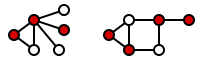
\includegraphics[height=0.2\textheight]{img/Vertex-cover}
\end{column}
\end{columns}
\end{frame}


\begin{frame}\frametitle{Max Clique }
\begin{columns} 
  \begin{column}{0.48\textwidth}
  \begin{block}{Instance}
    Undirected graph $G=\langle V,E \rangle$
  \end{block}
  \begin{block}{Feasible solution}
    Find a set $C\subset V$ such that all pairs of vertices in $C$ are connected by an edge
  \end{block}
    \begin{block}{Objective function}
      $|C|$
    \end{block}
  \end{column}
    
    \begin{column}{0.48\textwidth}
      \centering

  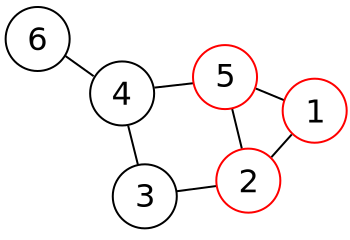
\includegraphics[height=0.5\textheight]{img/6n-graf-clique}
\end{column}
\end{columns}
\end{frame}

\begin{frame}\frametitle{Max Independent Set }
\begin{columns} 
  \begin{column}{0.48\textwidth}
  \begin{block}{Instance}
    Undirected graph $G=\langle V,E \rangle$
  \end{block}
  \begin{block}{Feasible solution}
    Find a set $I\subset V$ such that no two vertices in $K$ are connected by an edge
  \end{block}
    \begin{block}{Objective function}
      $|K|$
    \end{block}
  \end{column}
    
    \begin{column}{0.48\textwidth}
      \centering
  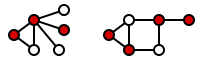
\includegraphics[height=0.2\textheight]{img/Vertex-cover}
\end{column}
\end{columns}
\end{frame}

\begin{frame}\frametitle{Max Cut }
\begin{columns} 
  \begin{column}{0.48\textwidth}
  \begin{block}{Instance}
    A weighted undirected  graph $G=\langle V,E \rangle$, $w:E\mapsto \mathbb{Q}^{+}$
  \end{block}
  \begin{block}{Feasible solution}
    a bipartition $(V_{1},V_{2})$ of $V$
  \end{block}
  \begin{block}{Objective function}
    $\sum_{v_{1}\in V_{1}, v_{2}\in V_{2}} w(v_{1}, v_{2})$
  \end{block}
\end{column}
    
    \begin{column}{0.48\textwidth}
      \centering
  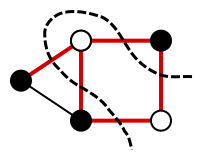
\includegraphics[height=0.7\textheight]{img/Max-cut}
\end{column}
\end{columns}
\end{frame}



\begin{frame}\frametitle{Min Traveling Salesperson (TSP)}
\begin{columns} 
  \begin{column}{0.48\textwidth}
  \begin{block}{Instance}
    A weighted undirected graph $G=\langle V,E \rangle$, $w:E\mapsto \mathbb{Q}^{+}$
  \end{block}
  \begin{block}{Feasible solution}
    Find a cycle $C$ that visits each vertex  $v\in V$ exactly once.
%
  \end{block}
  \begin{block}{Objective function}
    $\sum_{e\in C}w(e)$
  \end{block}
\end{column}
    \begin{column}{0.48\textwidth}
      \centering
  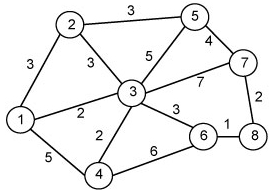
\includegraphics[height=0.5\textheight]{img/tsp}
\end{column}
\end{columns}
\end{frame}

\begin{frame}\frametitle{Approximation Goal }
  \begin{block}{Complexity classes}
    \begin{itemize}
    \item
      NPO: Optimization problems in NP
    \item
      FPTAS: Fully polynomial-time approximation scheme.
%
      Guaranteed error ratio $(1+\epsilon)$ or $(1-\epsilon)$, for any $\epsilon > 0$.
%
      Time complexity polynomial in $n$ and $\frac{1}{\epsilon}$
    \item
      PTAS: Polynomial-time approximation scheme.
%
      Guaranteed error ratio $(1+\epsilon)$ or $(1-\epsilon)$, for any $\epsilon > 0$.
%
      Time complexity polynomial in $n$ --- can be exponential in $\frac{1}{\epsilon}$,
      e.g. $O(n^{1/\epsilon})$
    \item
      APX: $O(1)$ approximation ratio, polytime
    \item
      MAX SNP: Definition based on logic and L-reduction.
%
      MAX SNP is included in APX
    \end{itemize}
  \end{block}
\end{frame}


\begin{frame}\frametitle{Min Set Cover }
\begin{columns} 
  \begin{column}{0.48\textwidth}
  \begin{block}{Instance}
    Universe set $U$, collection $\mathcal{S} = \{S_{1}, \ldots , S_{n}\}$of subsets of
    $U$.
    Weight $w: \mathcal{S}\mapsto \mathbb{Q}^{+}$
%
  \end{block}
  \begin{block}{Feasible solutions}
    A cover, that is a subcollection $\mathcal{C}$ of $\mathcal{S}$ that covers all elements of $U$
  \end{block}
  \begin{block}{Objective function}
    $\sum_{C\in \mathcal{C}} w(C)$
  \end{block}
\end{column}
    
    \begin{column}{0.48\textwidth}
      \centering

  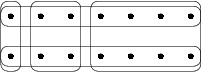
\includegraphics[height=0.2\textheight]{img/SetCoverGreedy}
\end{column}
\end{columns}
\end{frame}

\begin{frame}\frametitle{Min Set Cover }
\begin{columns} 
  \begin{column}{0.61\textwidth}
\begin{algorithm}[H]
  $C, D\gets \emptyset$\;
\While{$C\neq U$}
{
  $X\gets$ the set in $\mathcal{S}$ minimizing $w(X)/|X\setminus C|$\;
  $\alpha = \frac{w(X)}{|X\setminus C|}$\;
  Add $X$ to $D$\;
  For each $e\in C\setminus X$, $p(e)\gets \alpha$\;
  $C\gets C\cup X$
}
Output $D$
\caption{greedy-set-cover}
\end{algorithm}
\end{column}
  \begin{column}{0.34\textwidth}
\begin{block}{Lemma}
    $p(e_{k}) \le \frac{OPT}{n-k+1}$
  \end{block}
  \begin{block}{Corollary}
    Approximation factor is $1 + \frac{1}{2} + \frac{1}{3} + \cdots + \frac{1}{n} \le
    O(\log n)$
  \end{block}
\end{column}
\end{columns}
\end{frame}

\begin{frame}\frametitle{Min Metric Steiner Tree}
\begin{columns} 
  \begin{column}{0.48\textwidth}
  \begin{block}{Instance}
    A weighted undirected graph $G=\langle V,E \rangle$, $w:E\mapsto \mathbb{Q}^{+}$, $w$
    with triangle inequality.
%
    $V$ partition into $R$ (required) and $S$ (steiner)
  \end{block}
  \begin{block}{Feasible solution}
    A subtree $T$ of $G$ that includes all required vertices.
%
  \end{block}
  \begin{block}{Objective function}
    $\sum_{e\in T}w(e)$
  \end{block}
\end{column}
    \begin{column}{0.48\textwidth}
      \begin{block}{Approximation}
        Spanning tree $T$ of $G$
      \end{block}
      \begin{block}{2-approximation}
Euler tour of optimal solution $T^{*}$
      \end{block}
    \end{column}
\end{columns}
\end{frame}

\begin{frame}\frametitle{Min Metric Traveling Salesperson (TSP)}
\begin{columns} 
  \begin{column}{0.48\textwidth}
  \begin{block}{Instance}
    A weighted undirected graph $G=\langle V,E \rangle$, $w:E\mapsto \mathbb{Q}^{+}$, $w$
    with triangle inequality.
  \end{block}
  \begin{block}{Feasible solution}
    Find a cycle $C$ that visits each vertex  $v\in V$ exactly once.
%
  \end{block}
  \begin{block}{Objective function}
    $\sum_{e\in C}w(e)$
  \end{block}
\end{column}
    \begin{column}{0.48\textwidth}
      \begin{block}{2-approximation}
        Euler tour
      \end{block}
      \begin{block}{$\frac{3}{2}$-approximation}
Matching on odd-degree vertices of a spanning tree $T$
      \end{block}
    \end{column}
\end{columns}
\end{frame}

  \begin{frame}\frametitle{Shortest Superstring }
  \begin{block}{Instance}
      $s_{1}, \ldots, s_{m}$: strings of length $n$.
  \end{block}
  \begin{block}{Feasible solution}
    A superstring $T$, that is each $s_{i}$ is a substring of $T$
%
  \end{block}
  \begin{block}{Objective function}
    $|T|$
  \end{block}
\end{frame} 


  \begin{frame}\frametitle{Shortest Superstring }
  \begin{block}{Prefix graph}
      Arc $s_{i}, s_{j}$ with weight $pref(s_{i}, s_{j})$
  \end{block}
  \begin{block}{Length of superstring}
    Cycle of prefix graph + overlap last and first string
%
  \end{block}
  \begin{block}{Assignment problem = cycle cover}
    From $G=\langle V, E\rangle$ to $G_{2}$ with two copies $U$, $W$ of $V$.
%
    For each edge $(v_{i}, v_{j})\in E$, add two edges $(u_{i}, w_{i})$, $(w_{i}, u_{i})$
    to $G_{2}$
  \end{block}
  \begin{block}{Algorithm}
    \begin{itemize}
    \item
      Concatenate all cycle covers
    \item
      4-approximation
    \end{itemize}
  \end{block}
\end{frame} 


\begin{frame}\frametitle{Knapsack }
  \begin{block}{Instance}
    Universe set $U$, size $s: U \mapsto \mathbb{Z}^{+}$, profit $p: U \mapsto
    \mathbb{Z}^{+}$, capacity $B\in \mathbb{Z}^{+}$
%
  \end{block}
  \begin{block}{Feasible solutions}
    A subset $K\subseteq U$, such that $\sum_{k\in K}s(k) \le B$
  \end{block}
  \begin{block}{Objective function}
    $\sum_{k\in K} p(k)$, to maximize
  \end{block}
\end{frame}


\begin{frame}\frametitle{Knapsack }
  \begin{block}{Algorithm}
    \begin{itemize}[<.->]
    \item
      Dynamic programming
    \item
      NP-hard
    \item
      $K(i,b)$: uses only $\{u_{1}, \ldots, u_{i}\}$, total size $b$
    \item
      pseudo-polynomial time
    \item
      Transform it into an approximation algorithm
    \item
      Scale down profits $p_{1}(u) = \lfloor p(u) \frac{n}{\epsilon \max\{p(u)\}} \rfloor$, move to dual problem
    \item
      Approximation factor $1-\epsilon$, $\forall \epsilon>0$
    \item
      Time polynomial in $n$ and $\frac{1}{\epsilon}$
    \item
      \emph{FPTAS}
    \end{itemize}
  \end{block}
\end{frame} 

% \begin{frame}\frametitle{Bin Packing }
%   \begin{block}{Instance}
%     Universe set $U$, size $s: U \mapsto \mathbb{Q}^{+}$, $s(u)< 1 \forall u\in U$
% %
%   \end{block}
%   \begin{block}{Feasible solutions}
%     A partition $P$ of $U$ such that the sum $\sum_{u\in C} s(u) \le 1$ for each class
%   $C$ of the partition $P$
%   \end{block}
%   \begin{block}{Objective function}
%     the number of classes of $P$, to minimize
%   \end{block}
% \end{frame} 
\begin{frame}\frametitle{Linear Programming }
  \begin{block}{Basic facts}
    \begin{itemize}
    \item
      The primal has finite optimum iff the dual has finite optimum
    \item
      Let $x$, $y$ be two feasible solution of the primal and dual.
%
      Then $x$ are $y$ re both optimal if:
      \begin{enumerate}
      \item
        $\forall j$: either $x_{j}=0$ or $\sum_{i} a_{i,j}y_{i} = c_{j}$
      \item
        $\forall i$: either $y_{i}=0$ or $\sum_{j} a_{i,j}x_{j} = b_{i}$
      \end{enumerate}
    \end{itemize}
  \end{block}
\end{frame}

\begin{frame}\frametitle{Min Vertex Cover }
  \begin{block}{Integral version}
  \begin{equation}
    \begin{split}
      \min \sum x_{v} \qquad\text{subject to}\\
      x_{v} + x_{w} \ge 1\quad \forall (v,w)\in E\\
      x_{v}\in \{0,1\}\quad \forall v\in V
     \end{split}
   \end{equation}
 \end{block}
 \begin{block}{Fractional version}
  \begin{equation}
    \begin{split}
      \min \sum x_{v} \qquad\text{subject to}\\
      x_{v} + x_{w} \ge 1\quad \forall (v,w)\in E\\
      0\le x_{v}\le 1\quad \forall v\in V
     \end{split}
   \end{equation}
 \end{block}
\end{frame}


\begin{frame}\frametitle{Integrality ratio }
  \begin{equation}
    sup_{I} \frac{OPT(I)}{OPT_{f}(I)}
  \end{equation}

  over all instances $I$,
  where $OPT$ is the integral optimum, $OPT_{f}$ is the fractional optimum

  \begin{block}{Lemma}
    An LP-based approach cannot outperform the integrality ratio
  \end{block}
\end{frame}

\begin{frame}\frametitle{Half Integrality of Vertex Cover }
  \begin{block}{Fractional version}
  \begin{equation}
    \begin{split}
      \min \sum x_{v} \qquad\text{subject to}\\
      x_{v} + x_{w}\quad \forall (v,w)\in E\\
      x_{v}\ge 0 \quad \forall v\in V
     \end{split}
   \end{equation}
 \end{block}
 \begin{block}{Lemma}
     There exists an optimal solution with $x_{v}\in \{0, 1, \frac{1}{2}\}$
 \end{block}
\end{frame}

\begin{frame}\frametitle{Half Integrality of Vertex Cover }
 \begin{block}{Lemma}
     There exists an optimal solution with $x_{v}\in \{0, 1, \frac{1}{2}\}$
 \end{block}
\begin{columns}
  \begin{column}{0.04\textwidth}
      $y_{v} =$
  \end{column}
  \begin{column}{0.3\textwidth}
  \begin{equation}
    \begin{split}
      x_{v} +\epsilon, \frac{1}{2} < x_{v} < 1\\
      x_{v} -\epsilon, 0 < x_{v} < \frac{1}{2}
    \end{split}
  \end{equation}
\end{column}\hfill
  \begin{column}{0.04\textwidth}
      $z_{v} =$
  \end{column}
  \begin{column}{0.3\textwidth}
    \begin{equation}
    \begin{split}
      x_{v} -\epsilon, \frac{1}{2} < x_{v} < 1\\
      x_{v} +\epsilon, 0 < x_{v} < \frac{1}{2}
    \end{split}
  \end{equation}
\end{column}
\end{columns}
 \begin{block}{Proof}
   $x = \frac{1}{2}(y+z)$.
%
   Choose $\epsilon$ sufficiently small, then $y$ and $z$ are both feasible
 \end{block}
\end{frame}



\begin{frame}\frametitle{Dual Fitting for Greedy Set Cover }
\begin{columns} 
  \begin{column}{0.55\textwidth}
\begin{algorithm}[H]
  $C, D\gets \emptyset$\;
\While{$C\neq U$}%
{
  $X\gets$ set in $\mathcal{S}$ with min $w(X)/|X\setminus C|$\;
  $\alpha = \frac{w(X)}{|X\setminus C|}$\;
  Add $X$ to $D$\;
  For each $e\in C\setminus X$, $p(e)\gets \alpha$\;
  $C\gets C\cup X$
}
Output $D$
\end{algorithm}
\end{column}
  \begin{column}{0.41\textwidth}
  \begin{block}{ILP}
    \begin{equation}
    \begin{split}
      \min \sum_{S\in \mathcal{S}} w(S) \qquad\text{subject to}\\
      \sum_{S: e\in S} x_{S}\ge 1\quad \forall e\in U\\
      x_{S}\in \{0,1\}\quad \forall S\in \mathcal{S}
     \end{split}
   \end{equation}
 \end{block}
\end{column}
\end{columns}
\end{frame}


\begin{frame}\frametitle{Dual Fitting for Greedy Set Cover }
\begin{columns} 
  \begin{column}{0.48\textwidth}
  \begin{block}{Primal}
    \begin{equation}
    \begin{split}
      \min \sum_{S\in \mathcal{S}} w(S) \qquad\text{subject to}\\
      \sum_{S: e\in S} x_{S}\ge 1\quad \forall e\in U\\
      x_{S}\ge 0\quad \forall S\in \mathcal{S}
     \end{split}
   \end{equation}
 \end{block}
\end{column}
\begin{column}{0.48\textwidth}
  \begin{block}{Dual}
    \begin{equation}
    \begin{split}
      \max \sum_{e\in U} y_{e} \qquad\text{subject to}\\
      \sum_{e: e\in S} y_{e}\le c(S)\quad \forall S\in \mathcal{S}\\
      y_{e}\ge 0\quad \forall S\in \mathcal{S}
     \end{split}
   \end{equation}
 \end{block}
\end{column}
\end{columns}

\centering
 \begin{block}{Algorithm --- ILP}
   $p(e) = y_{e}$
 \end{block}
 Not dual feasible
\end{frame}

\begin{frame}\frametitle{Dual Fitting for Greedy Set Cover }
 \begin{block}{Fitting}
   $y_{e} = \frac{p(e)}{H_{n}}$,  $H_{n} = \sum_{i=1}^{n} \frac{1}{i}$
 \end{block}
 \begin{block}{Lemma}
   $x$, $y$ are both feasible
 \end{block}
 \begin{block}{Proof}
   Let $S\in \mathcal{S}$, $|S|=k$.
%
   Let $e_{1}, \ldots , e_{k}\in S$, same order as the algorithm.
%
   When inserting $e_{i}$, there are are least $k-i+1$ uncovered elements of $S$.
%
   By choice of $S$, $p(e_{i})\le c(S)/(k-i+1)$, hence $y_{e} = \frac{p(e_{i})}{H_{n}}\le
   \frac{c(S)/(k-i+1)}{H_{n}}$.
   Checking the constraint: $\sum_{i=1}^{k}y_{e_{i}} \le  \frac{c(S)}{H_{n}}
   \sum_{i=1}^{k}\frac{1}{i} = c(S)$
 \end{block}
 % 
 \end{frame}

 

\begin{frame}\frametitle{Max Cut}
  \begin{block}{Integral version}
  \begin{equation}
    \begin{split}
      \max \frac{1}{2}\sum_{i,j} w_{i,j}d_{i,j}\qquad\text{subject to}\\
      d_{i,j} \le x_{i} + x_{j} \quad \forall (v_{i}, v_{j})\in E\\
      d_{i,j} \le 2 - \left(x_{i} + x_{j}\right) \quad \forall (v_{i}, v_{j})\in E\\
      x_{v}, d_{i,j}\in \{0,1\}
     \end{split}
   \end{equation}
 \end{block}
\end{frame}

\begin{frame}\frametitle{Max Cut}
\begin{columns} 
  \begin{column}{0.48\textwidth}
  \begin{block}{Second version}
  \begin{equation}
    \begin{split}
      \max \frac{1}{2}\sum_{i,j} w_{i,j}(1 - x_{i}x_{j})\qquad\text{subject to}\\
      x_{v}^{2} =1\quad \forall v\in V\\
      x_{v}, d_{i,j}\in \{0,1\}
     \end{split}
   \end{equation}
 \end{block}
\end{column}
  \begin{column}{0.48\textwidth}
\begin{block}{Fractional version}
  \begin{equation}
    \begin{split}
      \max \frac{1}{2}\sum_{i,j} w_{i,j}(1 - x_{i}x_{j})\qquad\text{subject to}\\
      x_{v}^{2} =1\quad \forall v\in V\\
      -1\le x_{v}\le  1\quad \forall v\in V
     \end{split}
   \end{equation}
 \end{block}
\end{column}
\end{columns}
\end{frame}

\begin{frame}\frametitle{Semidefinite programming}
  \begin{block}{Vector version}
  \begin{equation}
    \begin{split}
      \max \frac{1}{2}\sum_{i,j} w_{i,j}(1 - x_{i}\cdot x_{j})\qquad\text{subject to}\\
      x_{v} \cdot x_{v} =1\quad \forall v\in V\\
      x_{v}\in \mathbb{R}^{n}\quad \forall v\in V
     \end{split}
   \end{equation}
 \end{block}
  \begin{block}{How to solve?}
    Can be solved approximately (additive error $\epsilon$) via interior point
  \end{block}
  \begin{block}{Problem}
    From vector (fractional) solution to bipartition
  \end{block}
\end{frame}

\begin{frame}\frametitle{Semidefinite programming}
  \begin{block}{Solution}
    \begin{itemize}
      \item
        Random hyperplane
      \item
        Contribution of vertices $x_{i}$, $x_{j}$ is $\frac{w_{i,j}}{2}\left( 1 - cos
          \theta_{i,j}\right)$, where $\theta_{i,j}$ is the angle between the two vectors
        $x_{i}$, $x_{j}$
      \item
        Probability of separation: $\frac{\theta_{i,j}}{\pi}$
      \end{itemize}
    \end{block}
  \begin{block}{Approximation Factor}
    \begin{equation}
      \alpha = \frac{2}{\pi} \min_{\theta} \frac{\theta}{1- cos \theta} > 0.878
    \end{equation}
  \end{block}
\end{frame}


% \begin{frame}\frametitle{Min $k$-Cut }
%   \begin{block}{Instance}
%     A weighted undirected  graph $G=\langle V,E \rangle$, $w:V\mapsto \mathbb{Q}^{+}$
%   \end{block}
%   \begin{block}{Feasible solution}
%     a $k$-partition $(V_{1},\ldots ,V_{k})$ of $V$
%   \end{block}
%   \begin{block}{Objective function}
%     $\sum_{v\in V_{i}, u\in V_{j}, i\neq j} w(v,u)$
%   \end{block}
% \end{frame}

\begin{frame}\frametitle{Max Sat}
\begin{columns} 
  \begin{column}{0.48\textwidth}
  \begin{block}{Instance}
    A set of boolean clauses $C=\{c_{1}, \ldots, c_{m}\}$ made of disjunctions over
  variables $X=\langle x_{1}, \ldots, x_{n}\rangle$
%
  A weight $w:C\mapsto \mathbb{Q}^{+}$ of each clause.
%
  \end{block}
  \begin{block}{Feasible solution}
    A truth assignment $Y$ to  the variables in $X$
  \end{block}
  \begin{block}{Objective function}
    $\sum_{c\in D} w(c)$, where $D$ is the set of clauses of $C$ that are made true by $Y$
  \end{block}
\end{column}
    
    \begin{column}{0.4\textwidth}
      \begin{block}{Example}
        $c_{1} = x_{1} \vee x_{3} \vee \neg x_{5}$\\
        $c_{2} = \neg x_{1} \vee \neg x_{2}$\\
        $c_{3} = x_{4}$
      \end{block}
    \end{column}
\end{columns}
\end{frame}


\begin{frame}\frametitle{Probabilistic Approach for Max Sat}
  \begin{block}{Random assignment}
    \begin{itemize}
    \item
      Each variable $x_{i}$ is true is probability $1/2$
    \item
      $E[w(c)] = w(c) \cdot Pr[c\text{ is satisfied}]$
    \item
      Depends on $size(c) = k_{c}$
    \item
      $E[w(c)] = w(c) \left( 1 - 2^{-k_{c}}\right) = \alpha_{k} w_{c}$, for $\alpha_{k} =
      \left( 1 - 2^{-k_{c}}\right)$
    \item
      Since $\alpha_{k}\ge \frac{1}{2}$, then $\frac{1}{2}-approximation$ (expected)
    \end{itemize}
  \end{block}
\end{frame}
  

\begin{frame}\frametitle{Conditional expectation}
  \begin{block}{Derandomize}
    \begin{enumerate} 
    \item
      $E[Y] = \sum_{c\in C} \alpha_{k} w_{c}$
    \item
      $E[Y] = \frac{1}{2} \left(E[Y|x_{1} = T] +E[Y|x_{1} = F] \right)$
    \item
      Pick the best between $E[Y|x_{1} = T]$ and $E[Y|x_{1} = F]$
    \end{enumerate}
  \end{block}
\end{frame}

\begin{frame}\frametitle{LP Approach for Max Sat}
  \begin{block}{ILP for Max Sat}
  \begin{equation}
    \begin{split}
      \max_{c\in C}w_{c}z_{c}\qquad\text{subject to}\\
      \sum_{i\in S_{c}^{+}}y_{i} + \sum_{i\in S_{c}^{-}}(1 - y_{i})\ge z_{c}\quad \forall c\in C\\
      y_{i}\in \{0, 1\}\quad \forall i\\
      z_{c}\in \{0, 1\}\quad \forall c\in C
     \end{split}
   \end{equation}
   $S_{c}^{+}$: boolean variables non-negated in $c_{i}$,  $S_{c}^{-}$: boolean variables negated in $c_{i}$
 \end{block}
\end{frame}

\begin{frame}\frametitle{LP Approach for Max Sat}
\begin{columns} 
  \begin{column}{0.48\textwidth}
\begin{block}{ILP relaxation}
  \begin{equation}
    \begin{split}
      \max_{c\in C}w_{c}z_{c}\qquad\text{subject to}\\
      \sum_{i\in S_{c}^{+}}y_{i} + \sum_{i\in S_{c}^{-}}(1 - y_{i})\ge z_{c}\quad \forall c\in C\\
      0 \le y_{i}\le 1\quad \forall i\\
      0\le z_{c}\le 1\quad \forall c\in C
     \end{split}
   \end{equation}
 \end{block}
 $y^{*}, z^{*}$: fractional optimum
\end{column}
  \begin{column}{0.48\textwidth}
    \begin{block}{Algorithm}
      $x_{i}\gets T$ with probability $y_{i}^{*}$
    \end{block}
    \begin{block}{Lemma}
      $E[W] \ge \beta_{k} w_{c}z_{c}^{*}$, with $\beta_{k}=1- \left(1- \frac{1}{k}\right)^{k}$
    \end{block}
    \begin{block}{Proof}
      \begin{itemize}
      \item
   $c_{i}$ satisfied if at least a variable is $T$
      \item
        $E[W_{c}] = 1- \Pi_{i=1}^{k}(1-y_{i}) \ge 1 - \left(\frac{\sum_{i=1}^{k}(1 -
            y_{i})}{k}\right)^{k} \ge 1 - \left(1 - \frac{z_{c}^{*}}{k}\right)^{k}$
      \item
        $1 - \left(1 - \frac{z_{c}^{*}}{k}\right)^{k} \ge \beta_{k}$ for $0\le
        z_{c}^{*}\le 1$
      \end{itemize}
    \end{block}
  \end{column}
\end{columns}
\end{frame}


\begin{frame}\frametitle{LP Approach for Max Sat}
\begin{block}{Approximation}
  $\beta_{k}=1- \left(1- \frac{1}{k}\right)^{k} \ge 1 - \frac{1}{e}$
\end{block}

\begin{block}{Notice}
  $\beta_{k}$ monotone increasing
\end{block}
\end{frame}

\begin{frame}\frametitle{Better approximation for Max Sat}
\begin{block}{Algorithm}
Pick the better of the solutions of the two algorithms
\end{block}
\begin{block}{Approximation Factor}
  \begin{itemize}
  \item
    $E[W_{c}] = \alpha_{k}w_{c} + \beta_{k}w_{c}z_{c}^{*}$
  \item
    $z_{c}^{*}\le 1$, hence $E[W_{c}] = \alpha_{k}w_{c}z_{c}^{*} + \beta_{k}w_{c}z_{c}^{*}
    = \left(\alpha_{k} + \beta_{k}\right) w_{c}z_{c}^{*}$
  \item
    Prove $\alpha_{k} + \beta_{k} \ge \frac{3}{4}$
  \item
    $\frac{3}{4}$-approximation
  \end{itemize}
\end{block}
\end{frame}

\begin{frame}\frametitle{Max multicommodity flow}
  \begin{block}{Instance}
    Undirected graph $G=\langle V,E \rangle$.
%
    Capacity $c_{e}$ for each edge $E$.
%
    A set $\{(s_{1}, t_{1}), \ldots , (s_{k}, t_{k})\}$ of source-sink pairs (commodity)
  \end{block}
  \begin{block}{Feasible solution}
    A flow that respects the maximum capacity and satisfies flow conservation.
%
  \end{block}
    \begin{block}{Objective function}
      $\sum_{(s_{i}, t_{i})}$ flow from $s_{1}$ to $t_{i}$
    \end{block}
\end{frame}


\begin{frame}\frametitle{Max multicommodity flow }
\begin{columns} 
  \begin{column}{0.48\textwidth}
  \begin{block}{Primal}
    \begin{equation}
    \begin{split}
      \max \sum_{p\in P} f_{p}\qquad\text{subject to}\\
      \sum_{p: e\in p} f_{p}\le c_{e}\quad \forall e\in E\\
      f_{p}\ge 0\quad \forall \text{ paths } p\in P
     \end{split}
   \end{equation}
 \end{block}
\end{column}
\begin{column}{0.48\textwidth}
  \begin{block}{Dual}
    \begin{equation}
    \begin{split}
      \min \sum_{e\in E} c_{e}d_{e} \qquad\text{subject to}\\
      \sum_{e\in p} d_{e}\ge 1\quad \forall p\in P\\
      d_{e}\ge 0\quad \forall e\in E
     \end{split}
   \end{equation}
 \end{block}
\end{column}
\end{columns}

\centering
\begin{block}{$d_{e}$}
  distance between vertices.
%
\end{block}
\begin{itemize}
\item
  Flow-cut duality
\item
  Pick a multicut $D$
\end{itemize}
\end{frame}

\begin{frame}\frametitle{Growing regions }
\begin{columns} 
  \begin{column}{0.48\textwidth}
  \begin{block}{Goal}
    \begin{itemize}
    \item
      No region contains a source-sink pair
    \item
      region centered on a source
    \item
      $c(R) \le \epsilon wt(R)$, where $c(R)$ is the capacity of the cut
    \end{itemize}
  \end{block}
  \begin{block}{Lemma}
    Radius $\le \frac{1}{2}$, the ball has no source-sink pair
  \end{block}
\end{column}
    \begin{column}{0.4\textwidth}
      \centering
  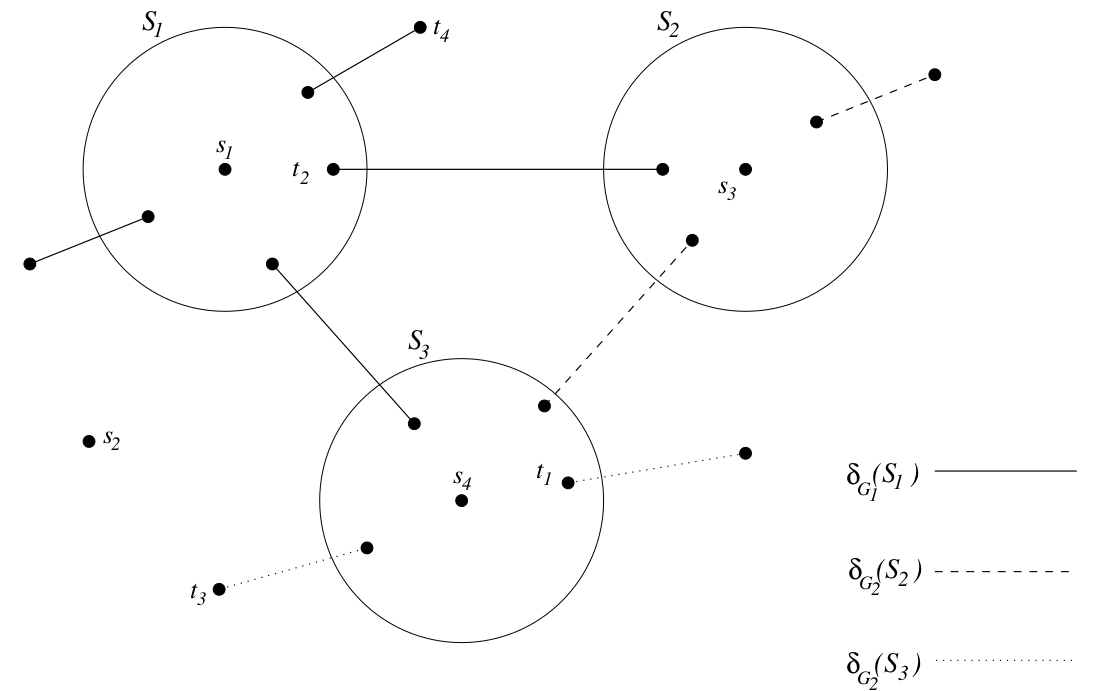
\includegraphics[height=0.5\textheight]{img/growing}
\end{column}
\end{columns}
\end{frame}

\begin{frame}\frametitle{Growing regions }
  \begin{block}{Weight distribution}
    \begin{itemize}
    \item
      $wt(s) = \frac{F}{k}$, with $s$ source, $F$ fractional optimum
    \item
      $q_{e}$: fraction of edge $e$ in the region
    \item
      $q_{e} = \frac{r - dist(s,u)}{dist(s,v) - dist(s,u)}$ for each edge $e=(u,v)$ in the cut
    \item
      $wt(R) = wt(s) + \sum_{e\in X} c_{e}d_{e}q_{e}$, with $X$ the set of edges with at
      least an endpoint in $R$
    \item
      Larger region $R$, easier $c(R) \le \epsilon wt(R)$
    \item
      $\epsilon \gets 2\ln (k+1)$ $\Rightarrow$ radius $\le \frac{1}{2}$
    \item
      $\frac{d wt(s(r))}{dr} \ge \sum_{e} c_{e}d_{e}\frac{d q_{e}}{dr} \ge c(S(r))$
    \end{itemize}
  \end{block}
\end{frame}

\begin{frame}\frametitle{Smooth polynomial programming }
\begin{columns} 
  \begin{column}{0.58\textwidth}
  \begin{block}{Program}
    \begin{equation}
    \begin{split}
      \max p(x_{1}, \ldots, x_{n})\qquad\text{subject to}\\
      \sum l_{i} \le p(x_{1}, \ldots, x_{n}) \le g_{i}\\
      x_{i}\in \{0, 1\}\quad \forall x_{i}
     \end{split}
   \end{equation}
 \end{block}
\end{column}
  \begin{column}{0.38\textwidth}
\begin{block}{Smoothness}
   For each degree-$d$ polynomial, each coefficient of each degree $i$ monomial is $\le c
   n^{d-i}$
 \end{block}
\end{column}
\end{columns}
\begin{block}{Compute a (random) solution with}
   \begin{itemize}
   \item
     Additive error $\epsilon n^{d}$
   \item
     degree-$f$ constraints satisfied with additive error $\epsilon n^{f}$
   \item
     linear constraints satisfied with additive error $O(\epsilon \sqrt{n \log n})$
   \item
     time complexity $O\left(\left(dKn^{d}\right)^{t}\right)$, with
     $t=4\frac{c^{2}e^{2}d^{2}}{\epsilon^{2}}$ and $K$ the number of constraints
   \end{itemize}
 \end{block}
\end{frame}

\begin{frame}\frametitle{Max Cut }
\begin{columns} 
  \begin{column}{0.48\textwidth}
  \begin{block}{Instance}
    A weighted undirected  graph $G=\langle V,E \rangle$, $w:E\mapsto \mathbb{Q}^{+}$
  \end{block}
  \begin{block}{Feasible solution}
    a bipartition $(V_{1},V_{2})$ of $V$
  \end{block}
  \begin{block}{Objective function}
    $\sum_{v_{1}\in V_{1}, v_{2}\in V_{2}} w(v_{1}, v_{2})$
  \end{block}
\end{column}
\begin{column}{0.48\textwidth}
  \begin{block}{Program}
    \begin{equation}
    \begin{split}
      \max_{(i,j)\in E} w(i,j)\left(x_{i}(1-x_{j})\right) + \left(x_{i}(1-x_{j})\right)%\qquad\text{subject to}\\
      % \sum l_{i} \le p(x_{1}, \ldots, x_{n}) \le g_{i}\\
      % x_{i}\in \{0, 1\}\quad \forall x_{i}
     \end{split}
   \end{equation}
 \end{block}
\end{column}
\end{columns}
\end{frame}

\begin{frame}\frametitle{Dense-$k$-subgraph }
\begin{columns} 
  \begin{column}{0.48\textwidth}
  \begin{block}{Instance}
    An undirected  graph $G=\langle V,E \rangle$
  \end{block}
  \begin{block}{Feasible solution}
    A subset $S$ of $k$ vertices of $G$
  \end{block}
  \begin{block}{Objective function}
    $|E\cap S\times S|$
  \end{block}
\end{column}
\begin{column}{0.48\textwidth}
  \begin{block}{Denseness}
    Average degree $\delta$%
 \end{block}
  \begin{block}{Random algorithm}
    Has $\alpha^{2} \delta^{2} n^{2}/2$ edges.
%
 \end{block}
\end{column}
\end{columns}
\end{frame}

\begin{frame}\frametitle{Dense-$k$-subgraph }
\begin{columns} 
  \begin{column}{0.48\textwidth}
  \begin{block}{Instance}
    An undirected  graph $G=\langle V,E \rangle$
  \end{block}
  \begin{block}{Feasible solution}
    A subset $S$ of $k$ vertices of $G$
  \end{block}
  \begin{block}{Objective function}
    $|E\cap S\times S|$
  \end{block}
\end{column}
\begin{column}{0.48\textwidth}
  \begin{block}{Program}
    \begin{equation}
    \begin{split}
      \max_{(i,j)\in E} x_{i}x_{j}\qquad\text{subject to}\\
      \sum x_{i} = k\\
      x_{i}\in \{0, 1\}\quad \forall x_{i}
     \end{split}
   \end{equation}
 \end{block}
 \begin{block}{Linear constraint}
   Move $O(\sqrt{n \log n})$ vertices in/out the set $S$, at most $O(n\sqrt{n \log n}) = o(n^{2})$ edges affected
%
 \end{block}
\end{column}
\end{columns}
\end{frame}

\begin{frame}\frametitle{Attribution}
\small
  \begin{itemize}[<.->]
  \item
    Vertex Cover figure: By Miym - Own work, CC BY-SA 3.0,
    \url{https://commons.wikimedia.org/w/index.php?curid=6017739}
  \item
    Clique figure: Public Domain,
    \url{https://commons.wikimedia.org/w/index.php?curid=1072101}
  \item
    Max Cut figure: By Miym - Own work, CC BY-SA 3.0,
    \url{https://commons.wikimedia.org/w/index.php?curid=6002348}
  \item
    Set Cover figure: Public Domain, \url{https://commons.wikimedia.org/w/index.php?curid=647030}
  \end{itemize}
\end{frame}

\end{document}
%%% Local Variables:
%%% mode: latex
%%% TeX-PDF-mode: t
%%% buffer-file-coding-system: utf-8
%%% End:
